\newcommand\CodingSpectator{\textsc{CodingSpectator}}

\newcommand\CodingTracker{\textsc{CodingTracker}}

\newcommand\Performed{\texttt{performed}}

\newcommand\Canceled{\texttt{canceled}}

\newcommand\Unavailable{\texttt{unavailable}}

\Def{NumberOfEclipseAutomatedRefactorings}{33}

\Def{NumberOfCodingSpectatorSupportedRefactorings}{23}

\subsection{\CodingSpectator}

\CodingSpectator~\cite{CodingSpectatorWebPage, VakilianETAL2011Richer,
VakilianETAL2012UseDisuseMisuse, VakilianETAL2013Compositional} is an extensible
framework for collecting Eclipse usage data. Although researchers at the
University of Illinois at Urbana-Champaign developed \CodingSpectator{}
primarily for collecting detailed data about the use of Eclipse refactoring
tool, it also provides a reusable infrastructure for \emph{submitting usage
data} from users to a central repository.
\CodingTracker~\cite{NegaraETAL2012Dangerous, NegaraETAL2013ManualRefactorings,
CodingTrackerWebPage} is another data collector developed at Illinois, which
reuses the data submission infrastructure provided by \CodingSpectator.

\subsubsection{What Data Is Collected}

\CodingSpectator{} was designed for capturing detailed data about the use of
automated refactorings. It collects three kinds of refactoring events:
\Canceled, \Performed, and \Unavailable. If a programmer starts an automated
refactoring but quits it before it finishes, \CodingSpectator{} records a
\Canceled{} refactoring event. If a programmer applies an automated refactoring,
\CodingSpectator{} records a \Performed{} refactoring event. Finally, if
programmer invokes an automated refactoring but the IDE refuses to start the
automated refactoring saying that the refactoring is not applicable to the
selected program element, \CodingSpectator{} records an \Unavailable{}
refactoring event.

Eclipse creates a \emph{refactoring descriptor} object for each \Performed{}
refactoring events and serializes it in an XML file. \CodingSpectator{} saves
more data in Eclipse refactoring descriptors of \Performed{} refactorings. In
addition, it creates and serializes refactoring descriptors for \Canceled{} and
\Unavailable{} refactoring events. \CodingSpectator{} supports
\Use{NumberOfCodingSpectatorSupportedRefactorings} of the
\Use{NumberOfEclipseAutomatedRefactorings} automated refactorings that Eclipse
supports.

We show a concrete example of the data that \CodingSpectator{} collects for an
invocation of the automated Extract Method refactoring. Eclipse provides an
automated refactoring called Extract Method for extracting a piece of code into
a new method. This refactoring moves the selected piece of code into a new
method and replaces the selected code by an invocation to the new method. To use
an automated Extract Method refactoring, a programmer has to go through multiple
steps. First, the programmer selects a piece of code
(\FigRef{FigCodingSpectatorExtractMethodSelectionExample}). Second, the
programmer invokes the automated Extract Method and configures it
(\FigRef{FigCodingSpectatorExtractMethodConfigurationExample}). In this case,
the programmer sets the name of the new method. The configuration page provides
a number of other options including method accessibility, the ordering and names
of method parameters, and the generation of method comments. Third, after
configuring the refactoring, the programmer hits the ``Preview'' button and the
automated refactoring reports the problems that the refactoring may introduce
(\FigRef{FigCodingSpectatorExtractMethodErrorExample}). In this example, the
automated refactoring complains that the selected name of the new method
conflicts with the name of an existing method. Finally, the programmer decides
to cancel the refactoring and \CodingSpectator{} records a refactoring
descriptor for this \Canceled{} refactoring as shown in
\FigRef{FigCodingSpectatorDescriptorExample}. The type of a refactoring event
(\ie, \Unavailable, \Canceled, and \Performed) can be inferred from the
directory in which the XML file containing the refactoring descriptor resides.
\CodingSpectator{} captures the following attributes for the canceled automated
Extract Method refactoring in the above example.

\begin{enumerate}

\item \texttt{captured-by-codingspectator}: indicates that \CodingSpectator{}
  created the refactoring descriptor.

\item \texttt{stamp}: a timestamp recording when the refactoring event occurred

\item \texttt{code-snippet}, \texttt{selection},
  \texttt{selection-in-code-snippet}, \texttt{selection-text}: the location and
  contents of the selection that the programmer made before invoking the
  automated refactoring

\item \texttt{id}: the automated refactoring's identifier

\item \texttt{comment}, \texttt{description}, \texttt{comments},
  \texttt{destination}, \texttt{exceptions}, \texttt{flags}, \texttt{input},
  \texttt{name}, \texttt{visibility}: configuration options, \eg{} input
  elements, project, and settings that programmers can set to control the effect
  of the refactoring

\item \texttt{status}: any problems reported by the automated refactoring to the
  programmer

\item \texttt{navigation-history}: when the programmer pressed a button to
  navigate from one page of the refactoring wizard to another

\item \texttt{invoked-through-structured-selection},
  \texttt{invoked-by-quick-assist}: selection method (\eg{} structured or
  textual selection and whether the automated refactoring was invoked using
  Quick Assist

\end{enumerate}

\begin{figure}
%
\centering
%
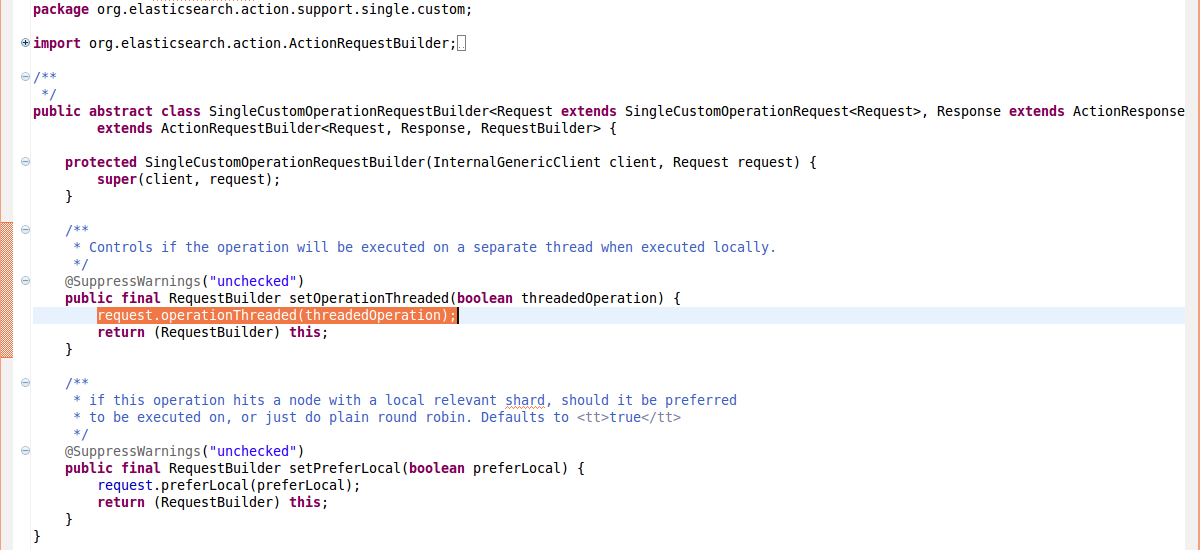
\includegraphics[width=\textwidth]{codingspectator-extract-method-selection.png}
%
\caption{\label{FigCodingSpectatorExtractMethodSelectionExample}A programmer
selects a piece of code to extract into a new method. The selected code is part
of class \texttt{SingleCustomOperationRequestBuilder} from commit
\texttt{bdb1992} of the open-source Elasticsearch project
(\texttt{https://github.com/elasticsearch/elasticsearch}).}
%
\end{figure}

\begin{figure}
%
\centering
%
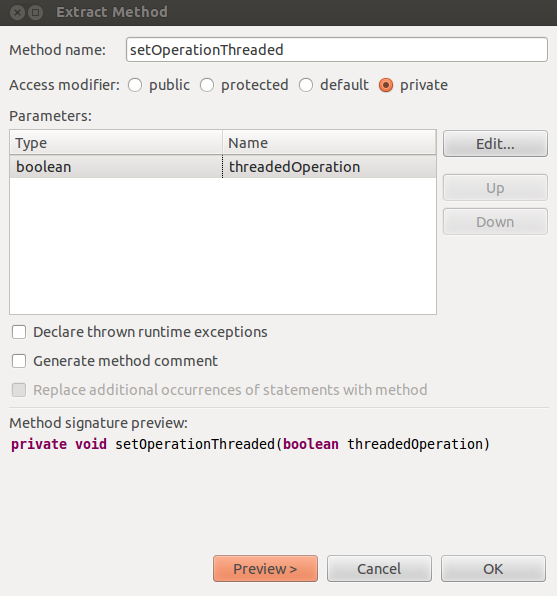
\includegraphics[width=0.5\textwidth]{codingspectator-extract-method-configuration.png}
%
\caption{\label{FigCodingSpectatorExtractMethodConfigurationExample}A programmer
configures an automated Extract Method refactoring by entering the desired name
of the new method.}
%
\end{figure}

\begin{figure}
%
\centering
%
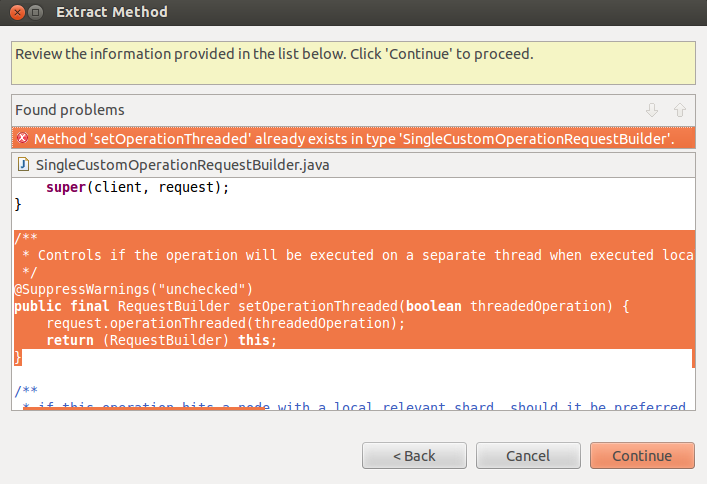
\includegraphics[width=0.6\textwidth]{codingspectator-extract-method-error.png}
%
\caption{\label{FigCodingSpectatorExtractMethodErrorExample}The Extract Method
refactoring reports a name conflict problem to the programmer. The programmer
can either ignore the problem and continue the refactoring, go back to the
configuration page to provide a different name, or cancel the refactoring.}
%
\end{figure}

\begin{figure}
%
\centering
%
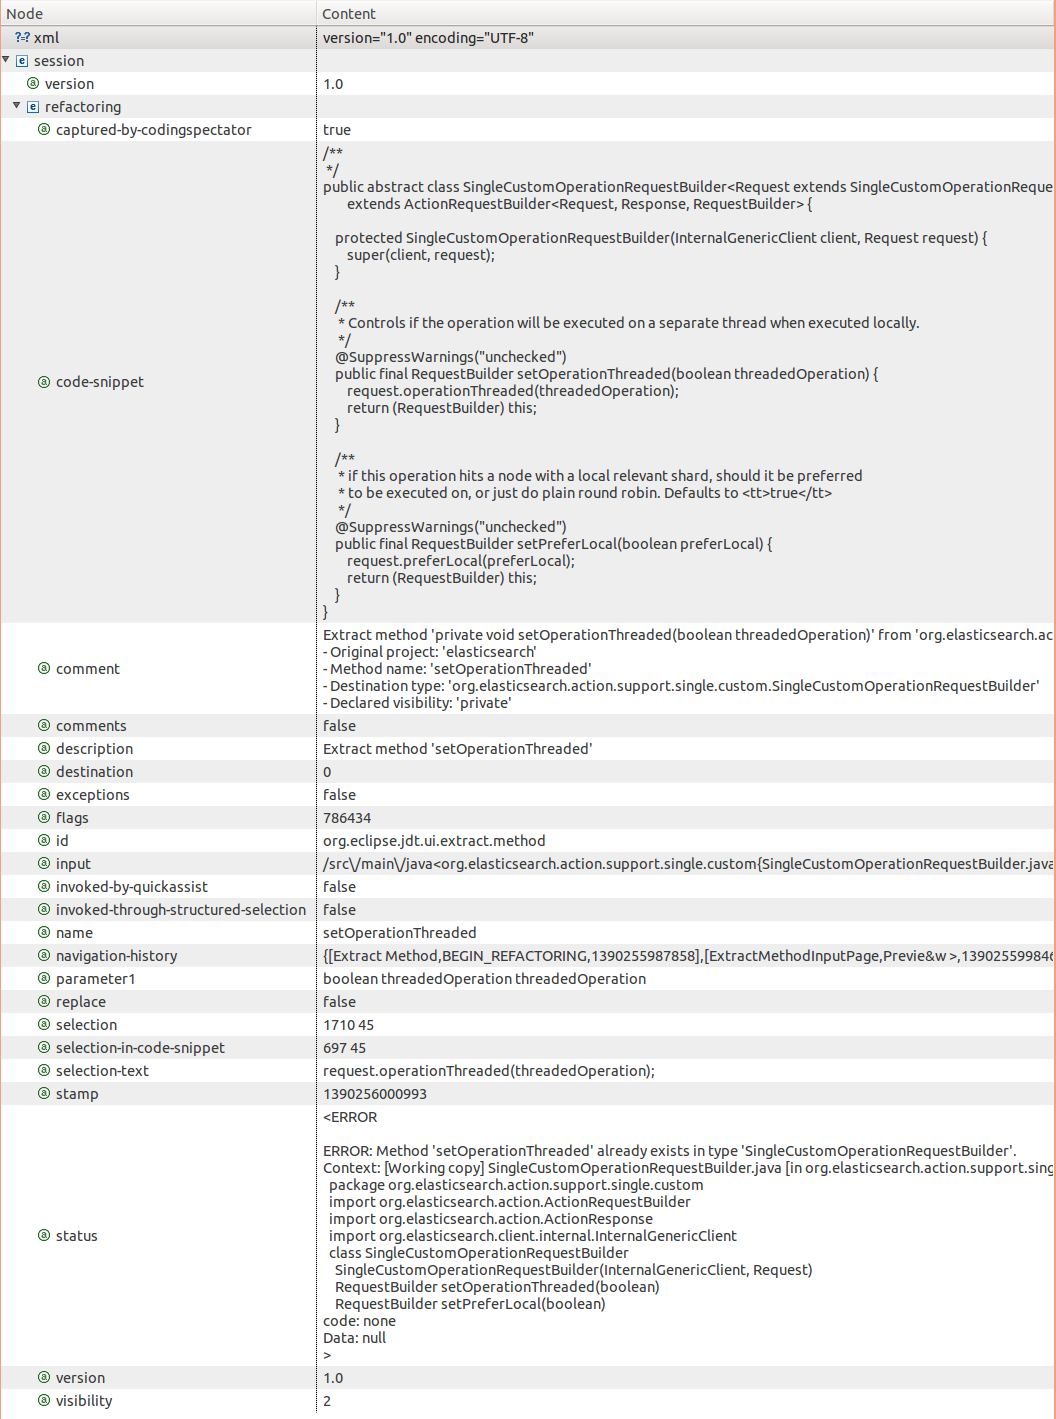
\includegraphics[width=\textwidth]{codingspectator-refactoring-xml.png}
%
\caption{\label{FigCodingSpectatorDescriptorExample}An example refactoring
descriptor recorded by \CodingSpectator.}
%
\end{figure}

\subsubsection{Deploying \CodingSpectator}

Deploying \CodingSpectator{} consists of two main steps:
%
\begin{inparaenum}[(1)]
%
\item setting up a Subversion repository and
%
\item setting up an Eclipse update site.
%
\end{inparaenum}

\paragraph{Setting Up a Subversion Repository}

\CodingSpectator{} regularly submits users' data to a central Subversion
repository. To collect \CodingSpectator's data automatically, you need to set up
a Subversion repository and create accounts for your users. To allow the users
submit their data to the Subversion repository, you should grant them
appropriate write accesses to the repository.

Using a Version Control System such as Subversion as the data repository has
several advantages:

\begin{enumerate}
%
\item Subversion makes all revisions of each file easily accessible. This makes
  troubleshooting easier for researchers.
%
\item For textual files, Subversion submits only the \emph{changes} made to the
  files as opposed to the entire new file. This differential data submission
  leads to faster submissions.
%
\item There are libraries such as SVNKit\footnote{http://svnkit.com/} that
  provide an API for Subversion operations such as add, update, remove, and
  commit. \CodingSpectator{} uses SVNKit for submitting users' data to the
  central repository.
%
\item Setting up a Subversion server is a well-documented process. This avoids
  the burden of setting up a specialized server.
%
\end{enumerate}

On the other hand, a disadvantage of using Subversion as the data repository is
that it requires the users to maintain a copy of their data on their file
systems. The Subversion working copy on the users' systems takes \emph{space}
and can also cause \emph{merge conflicts}, \eg, if a user restores the contents
of the file system to an earlier version. To handle merge conflicts,
\CodingSpectator{} has built-in support for automatic conflict detection and
resolution. When \CodingSpectator{} detects a merge conflict, it removes the
user's data from the central repository and then submits the new data. Despite
removing the data from the central repository, the researchers can still locate
the merge conflicts and restore the data that was collected before the merge
conflicts.

\CodingSpectator{} prompts the users for their Subversion usernames and
passwords when \CodingSpectator{} is about to submit their data.
\CodingSpectator{} gives the users the option to save their passwords in Eclipse
securely. See \url{http://codingspectator.cs.illinois.edu/documentation} for
more information about the features of \CodingSpectator{} for users.

\paragraph{Setting Up an Eclipse Update Site}

Users of \CodingSpectator{} install it from an Eclipse update
site\footnote{\url{http://codingspectator.cs.illinois.edu/installation}}. An
Eclipse update site is an online repository of the JAR and configuration files
that Eclipse requires for installing a plug-in.

% LocalWords: CodingSpectator Urbana Champaign IDE timestamp
%
% LocalWords: CodingTracker refactoring refactorings refactoring's
%
% LocalWords: SVNKit URL username online API

